\documentclass[12pt,a4paper]{article}
%preamble
\usepackage{fancyhdr}
\usepackage{wrapfig}
\usepackage{enumerate}
\usepackage{graphicx}
\usepackage[a4paper, margin=1.0in]{geometry}
\setlength{\headheight}{15pt}

%set header & footer
\pagestyle{fancy}
\lhead{EE516: Project 01}
\rhead{Gaurav Kalra (20164593)}

\begin{document}
\section{Task 01}
Write a bash shell script that shows tree structure of the directories and files included in your own home directory.

\begin{figure}[!h]
	\centering
	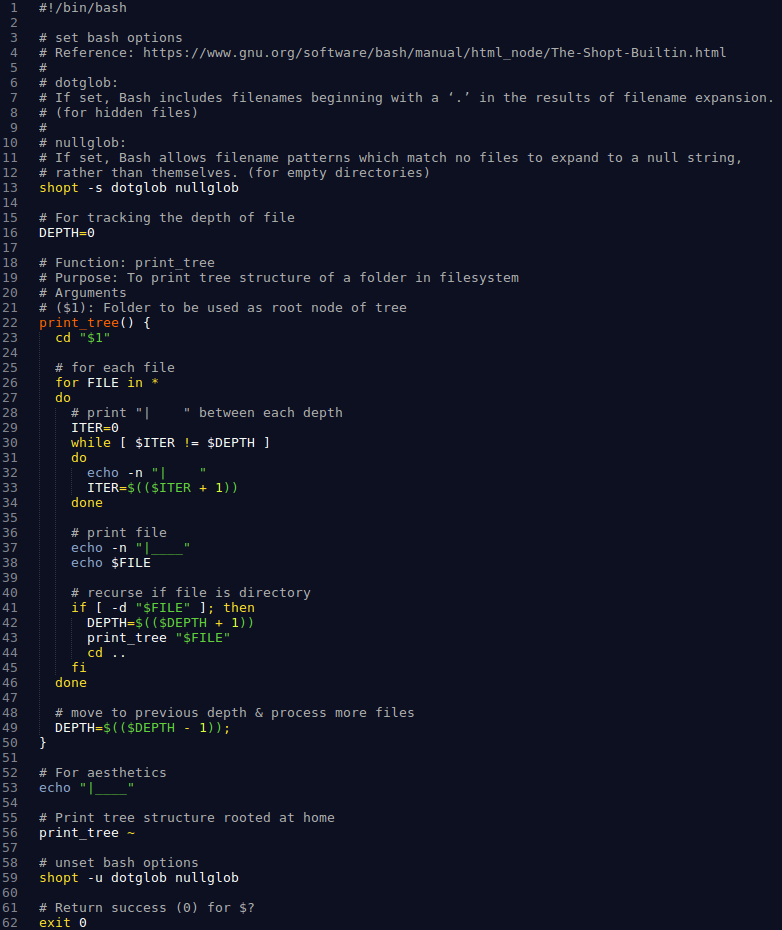
\includegraphics[width=6in]{./task01/task01.png}
	\caption{tree.sh}
\end{figure}

\newpage

\subsection{Key Points}
\begin{enumerate}
  \item Setting/Un-setting bash options
\begin{figure}[!h]
	
\includegraphics[width=2in]{./task01/task01_1_1.png}
	
\includegraphics[width=2in]{./task01/task01_1_2.png}
\end{figure}

\textbf{dotglob} instructs bash to include filenames beginning with a ``." in the results of filename expansion. \textbf{nullglob} allows filename patterns which match no files to expand to a null string, rather than themselves. These options are vital during execution of following \textit{for} loop:
\begin{figure}[!h]
	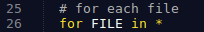
\includegraphics[width=1.5in]{./task01/task01_1_3.png}
\end{figure}

  \item Recursive implementation
\begin{figure}[!htb]
	
\includegraphics[width=1.5in]{./task01/task01_2_1.png}
	
\includegraphics[width=2in]{./task01/task01_2_2.png}
	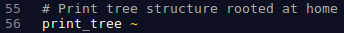
\includegraphics[width=2in]{./task01/task01_2_3.png}
\end{figure}

Function \textbf{print\_tree} is defined recursively parsing every directory from root node (home directory) to leaf node (file in a sub-directory).

  \item Handling filenames with whitespace(s)
\begin{figure}[!h]
	
\includegraphics[width=1in]{./task01/task01_3_1.png}
	
\includegraphics[width=2in]{./task01/task01_3_2.png}
	
\includegraphics[width=2in]{./task01/task01_3_3.png}
\end{figure}

It is important to enclose \textbf{\$1} and \textbf{\$FILE} with double-quotes since the variables may contain filenames having whitespace character.
\end{enumerate}

\begin{figure}[!h]
	\centering
	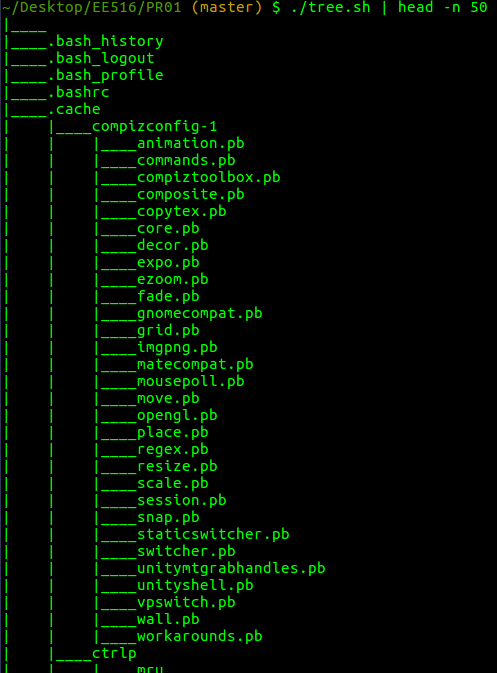
\includegraphics[width=2in]{./task01/task01_output.png}
	\caption{Snipped output of ./tree.sh}
\end{figure}

\end{document}